% Presentation (English) — The maximum length of a chess game under the
% FIDE Laws is 17,697 plies.
%
% Build:  tectonic slides-en.tex          (slides)
%         tectonic slides-en-notes.tex    (speaker script)
% Regenerate figures and screenshots:
%         uv run --with cairosvg --with playwright --with pymupdf \
%           python make_assets.py
%
% The slides state definitions, lemmas and proofs under the paper's own
% numbering, with a picture beside each.  What is said out loud lives in
% \note{}, which slides-en-notes.tex extracts.  Statement numbers are
% written by hand rather than counted: they must agree with main.tex, not
% with the order of the slides.  The figure vocabulary (\lcs*) defaults to
% English, so unlike the Korean deck this file needs no string table.
\documentclass[aspectratio=169,10pt]{beamer}
\usepackage{longchess}

\newcommand{\B}{\mathsf{B}}
\newcommand{\W}{\mathsf{W}}

\def\lcmapn{7}
\def\lcmapnames{{0.~Origin},{I.~Rules},{II.~Counting},{III.~Switches},%
  {IV.~Search},{V.~Checking},{VI.~Meaning}}

% Short forms feed Madrid's footline: author (institute) | title | date.
\title[The longest chess game]{The maximum length of a chess game\\
  under the FIDE Laws is 17{,}697 plies}
\author[Yim]{Junyeop Yim}
\institute[KNU]{Kongju National University}
\date[2026]{August 2026}

\begin{document}

\lctitleframe
\note{One sentence is the whole talk: the maximum length of a chess game is
exactly 17{,}697 plies. The value has been known since 2015; what was
missing is a proof that nothing is longer.}

% ========================================================== 0. Origin
\lcpart{0}{Origin}{a known value, and no proof}

\begin{frame}{Where the problem comes from}
  \centering
  \vspace{0.3cm}
  \begin{columns}[c]
    \begin{column}{0.36\textwidth}\centering
      \lcshot{5.0cm}{assets/shot-yt-video.jpg}{[YouTube thumbnail]}\\[3pt]
      \lccap{\textbf{Ing Chess}, developer of Augment Chess}
    \end{column}
    \begin{column}{0.05\textwidth}\centering
      {\Large\color{lcmid}$\rightarrow$}
    \end{column}
    \begin{column}{0.36\textwidth}\centering
      \lcshot{5.0cm}{assets/shot-labelle.png}{[wismuth.com capture]}\\[3pt]
      \lccap{F.~Labelle, \emph{The longest possible chess game}, 2015}
    \end{column}
  \end{columns}
  \par\vspace{0.55cm}
  \lcquote{``\emph{I believe} that the length of the longest possible
    chess game is $8848.5$ moves.''}{Labelle 2015}
  \note{The starting point was a video by Ing Chess, the developer of
  Augment Chess, a chess-variant web game: ``the theoretically longest
  chess game''.

  Its description links to François Labelle's page, and that page has
  essentially everything: the 118 delay plies, a three-switch schedule, a
  complete generated game.

  And the conclusion reads ``I believe''. The value was known; the proof was
  not. This talk is that proof.}
\end{frame}

\begin{frame}{Outline}
  \centering
  \lcmap{0}
  \par\vspace{0.85cm}
  {\small
  \begin{tabular}{@{}ll@{}}
    \textbf{I--III} & the upper bound --- hand-checkable combinatorics \\[4pt]
    \textbf{IV--V}  & computation --- the search that preceded it, and the
                      checking \\[4pt]
    \textbf{VI}     & what the result means \\
  \end{tabular}}
  \par\vspace{0.75cm}
  \lcquote{$L \;\le\; 150 \cdot 118 - 3 \;=\; \mathbf{17{,}697}$}{}
  \note{Seven parts, deliberately different in kind.

  Parts I to III are pure mathematics and no computer appears in them.
  Parts IV and V are entirely about computation --- the search that failed,
  and how the result was checked. Part VI is what it means.

  Everything lands on that one line: a hundred and eighteen segments of a
  hundred and fifty, minus three. That minus three is the paper.

  Statement numbers on these slides are the paper's own, so you can find any
  of them afterwards.}
\end{frame}

% ========================================================== I. Rules
\lcpart{I}{Rules}{in 2014, chess became finite}

\begin{frame}{The automatic terminations --- in force since 1 July 2014}
  \centering
  \lcmap{1}
  \par\vspace{0.45cm}
  \figrules
  \par\vspace{0.35cm}
  {\small Before 2014 the threefold-repetition and 50-move draws had to be
   \emph{claimed} --- two cooperating players could play forever
   (Euwe 1929, via Thue--Morse).}
  \note{Before 2014 the question had no finite answer. Threefold repetition
  and the 50-move rule both had to be claimed, so two cooperating players
  could play forever --- classically so, Euwe in 1929 by rediscovering the
  cube-free Thue--Morse sequence.

  Since 1 July 2014 the Laws end a game automatically. No claim.

  First: the same position five times. Second: 75 moves by each player with
  no pawn move and no capture --- the moment the clock reaches 150. Third is
  the dead-position article that was already there, and bare kings are its
  clearest instance.

  These rules have teeth. The seven-piece tablebases contain forced mates
  over five hundred moves long, and the second rule erases every one of
  them.

  From that moment the longest game is a well-posed problem in extremal
  combinatorics.}
\end{frame}

\begin{frame}{The halfmove clock $c(t)$}
  \centering
  \vspace{0.35cm}
  \figclock
  \par\vspace{0.55cm}
  {\small $c(t)$ = plies since the last pawn move or capture
   \quad$\cdot$\quad the reference game's first eleven segments, to scale}
  \note{This picture is half the talk: the first eleven segments of the
  actual reference game, drawn to scale.

  The vertical axis is the halfmove clock. A pawn move or a capture resets
  it to zero; anything else pushes it up by one. The moment it touches 150
  the game is over.

  So a long game must move a pawn or capture something just before the clock
  would reach 150. Each of those resets is a critical move --- Murphy's
  term; Labelle calls the same plies delay plies.

  Look at the right-hand end. Only the last segment lets the clock actually
  reach 150, and the ply that gets it there is checkmate. That ending is
  legal only because of the precedence clause.

  And segment eleven is 149. Why exactly one ply goes missing there is the
  whole of Part III.}
\end{frame}

\begin{frame}{Prior work}
  \centering
  \vspace{0.35cm}
  \figtimeline
  \par\vspace{0.85cm}
  \lcquote{``We clearly need at least one switch \dots\ but is it possible
    to do it with only two? If not, can this lower bound be proved?''}%
    {Murphy VII, SIGBOVIK 2020}
  \note{The question is older than the automatic rules. In the claim-based
  50-move setting chess problemists worked it out over half a century:
  Dawson published 5{,}900 in 1911, Fabel settled it at 5{,}898 and a half in
  1947.

  In 2004 Heimo wrote something remarkable: with an odd bound --- ``say
  75'' --- the answer would be White's 8{,}849th move. Ten years before the
  rule existed.

  The rule arrived in 2014. In 2015 Labelle assembled everything and wrote
  ``I believe''. In 2020 Murphy published a hand-built game, computed a
  ceiling of 17{,}699 from the construction, and closed with the quoted
  question.

  One switch is clearly needed, but can it be done with two? The answer
  today is no, and yes it can be proved.}
\end{frame}

\begin{frame}{The scale of $17{,}697$ plies}
  \centering
  \vspace{0.35cm}
  \begin{columns}[c]
    \begin{column}{0.52\textwidth}\centering
      \figscale
    \end{column}
    \begin{column}{0.44\textwidth}\centering
      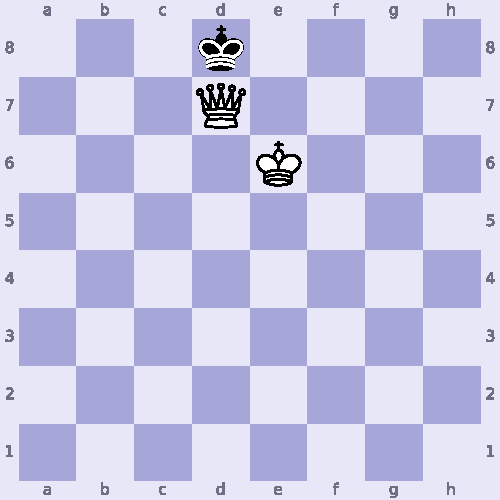
\includegraphics[height=3.1cm]{assets/board-witness}\\[4pt]
      {\small The final position --- king and queen against king}\\[2pt]
      {\scriptsize\color{lcaccent}
       The last ply is neither a pawn move nor a capture: a \emph{quiet}
       checkmate,\\ with the clock at exactly $150$}
    \end{column}
  \end{columns}
  \note{For scale. A tournament game runs about forty moves, eighty plies.
  One red cell on the left is that, and the longest game is two hundred and
  twenty-one of them end to end.

  On the right is where that game actually stops. King and queen against
  king. The last move is neither a pawn move nor a capture --- a quiet
  checkmate played at the exact moment the clock reads 150. Without the
  precedence clause it would have been a draw.}
\end{frame}

% ======================================================= II. Counting
\lcpart{II}{Counting}{$K \le 118$ --- counting suffices}

\begin{frame}{Definitions}
  \centering
  \lcmap{2}
  \par\vspace{0.4cm}
  \begin{columns}[t]
    \begin{column}{0.485\textwidth}
      \begin{lcstate}{Definition 2.1}{critical move}
        {\small A pawn move or a capture. (En passant is both; a promotion
        is a pawn move; castling is neither.) Any other move is
        \emph{quiet}.}
      \end{lcstate}
      \begin{lcstate}{Definition 2.2}{segments · endpoints}
        {\small Let the critical moves fall at plies $t_1<\dots<t_m$. Set
        $T=1$ if quiet plies follow the last of them, else $T=0$. The
        endpoints are $e_i=t_i$ and, if $T=1$, $e_{m+1}=L$; and
        $K=m+T$.}
      \end{lcstate}
    \end{column}
    \begin{column}{0.485\textwidth}
      \begin{lcstate}{Definition 2.3}{switches $S$}
        {\small The \emph{colour} of $e_i$ is the colour of whoever played
        that ply. The virtual endpoint $e_0=0$ is Black by convention.
        \[
          S=\#\{\,i\le K:\operatorname{col}(e_i)\ne
              \operatorname{col}(e_{i-1})\,\}.
        \]}
      \end{lcstate}
      \vspace{0.1cm}
      {\small Critical moves are exactly the moves that reset the clock,
      and they are \emph{irreversible} --- a pawn cannot retreat and a
      captured piece never returns.}
    \end{column}
  \end{columns}
  \note{Three definitions, numbered as in the paper.

  2.1. A critical move is a pawn move or a capture. En passant is both, a
  promotion is a pawn move, castling is neither. These coincide exactly with
  the moves that reset the clock, and their irreversibility is decisive
  later.

  2.2. The critical moves cut the game into segments. If quiet plies follow
  the last one, there is one closing segment more --- that is $T$ --- and
  the number of segments is $K$.

  2.3. The last ply of each segment is its endpoint, and its colour is
  whoever played it. $S$ counts how often that colour changes, measured
  against a virtual Black endpoint at the start of the game. Without that
  convention the first segment could not be counted at all.}
\end{frame}

\begin{frame}{Lemma 2.4 --- the segment decomposition}
  \centering
  \vspace{0.35cm}
  \begin{lcstate}{Lemma 2.4}{segment decomposition}
    \centering
    $L \;=\; 150K - S - \displaystyle\sum_{i=1}^{K}\delta_i,
     \qquad \delta_i \ge 0$\par\medskip
    {\small $\delta_i$ is segment $i$'s shortfall from its target length
    ($150$ if its endpoints share a colour, $149$ otherwise).
    In particular $L \le 150K - S$.}
  \end{lcstate}
  \vspace{0.2cm}
  \begin{lcproof}
    \begin{lcsteps}
      \item All plies of segment $i$ except possibly the last are quiet. If
        its length were $151$ or more, the first $150$ would all be quiet
        and the game would already have ended there (Art.~9.6.2) ---
        contradiction. So the length is $\le 150$.
      \item Plies alternate colour, so a segment's length is even exactly
        when its two endpoints share a colour. If they differ the length is
        odd, and being $\le150$ it is $\le149$.
      \item Summing the segment lengths telescopes to $e_K-e_0=L$.
        \qedhere
    \end{lcsteps}
  \end{lcproof}
  \note{Lemma 2.4 is the whole talk's ledger.

  The proof has three steps.

  Step one: a segment cannot exceed 150 plies. If it did, its first 150
  would all be quiet and 9.6.2 would already have ended the game there.

  Step two is where $S$ comes from, and the next slide shows it as a
  picture.

  Step three is a telescoping sum.

  The conclusion is $L \le 150K - S$. Now bound $K$ and $S$ separately.}
\end{frame}

\begin{frame}{Step (2) of Lemma 2.4 --- parity}
  \centering
  \vspace{0.35cm}
  \figparity
  \par\vspace{0.4cm}
  {\small Plies alternate colour $\;\Longrightarrow\;$ the parity of a
   segment's length is exactly whether its two endpoints share a colour}
  \note{This is pure parity.

  The picture uses the same idiom as the clock graph: over one segment the
  clock climbs and the final critical move drops it to zero. The strip below
  the axis is the colour of each ply.

  Top row: if the two endpoints share a colour, the number of plies between
  them is even. 150 is even, so the segment can be filled.

  Bottom row: if they differ, the length must be odd, and the largest odd
  number at most 150 is 149. So each colour change costs exactly one ply.

  That is the entire reason $S$ appears in the decomposition.}
\end{frame}

\begin{frame}{Counting the critical moves}
  \centering
  \vspace{-0.1cm}
  {\large $K \;=\; (P - O) \;+\; (C + T)$}
  \par\vspace{0.3cm}
  \figaccount
  \par\vspace{0.2cm}
  {\small $P$ pawn moves \quad $C$ captures \quad
   $O$ both at once \quad $T$ closing segment $\in\{0,1\}$}
  \note{Count the critical moves by inclusion--exclusion.

  A critical move is a pawn move or a capture, so the total is pawn moves
  plus captures minus the ones that are both. Those are the diagonal pawn
  captures, the overlaps $O$. Add one if there is a closing segment.

  The grouping matters: writing it as $P-O$ plus $C+T$ lets the two halves
  be bounded completely independently.

  And it has to hold for \emph{every} game. Reading ``eight overlaps, so 96
  minus 8'' off the known construction is circular --- whether that
  construction is optimal is exactly what we are proving. The next four
  slides do the work properly.}
\end{frame}

\begin{frame}{Lemma 3.1 --- one pawn's budget}
  \centering
  \vspace{0.2cm}
  \begin{columns}[c]
    \begin{column}{0.44\textwidth}\centering
      \figpawnfull
    \end{column}
    \begin{column}{0.53\textwidth}
      \begin{lcstate}{Lemma 3.1}{pawn basics}
        {\small Each pawn makes at most $6$ pawn moves, so $P \le 96$. A
        pawn that makes exactly $6$ advances exactly one rank each time and
        \emph{promotes}.}
      \end{lcstate}
      \begin{lcproof}
        {\small Every pawn move advances at least one rank, and there are
        six ranks between a pawn's home rank and the promotion rank. Six
        moves therefore means one rank each and arrival on the promotion
        rank, where promoting is compulsory. \qed}
      \end{lcproof}
    \end{column}
  \end{columns}
  \par\vspace{0.25cm}
  {\small\color{lcaccent}
   Corollary: $P = 96$ is equivalent to ``all $16$ pawns walked up one rank
   at a time, with no double push, and all $16$ promoted''.}
  \note{The easy one first. Six ranks between a pawn's home rank and
  promotion, and every pawn move advances at least one. So six per pawn,
  sixteen pawns, $P \le 96$.

  The corollary matters more. If a pawn made exactly six moves then each of
  them advanced exactly one rank --- no double pushes --- and it finished on
  the promotion rank, where promoting is compulsory.

  So $P = 96$ says: all sixteen pawns walked up one square at a time and all
  sixteen promoted. It also says no pawn is left on the board. We use it
  repeatedly.}
\end{frame}

\begin{frame}{Lemma 3.3 --- unresolved origin pairs}
  \centering
  \vspace{-0.05cm}
  \begin{columns}[c]
    \begin{column}{0.24\textwidth}\centering
      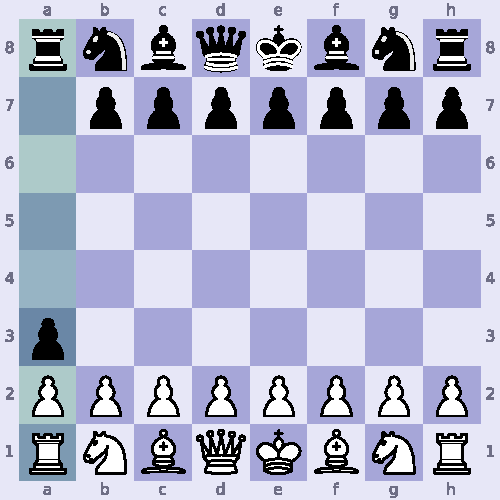
\includegraphics[width=\linewidth]{assets/board-cap10a}\\[2pt]
      \lccap{after 4\ldots a3: four Black}
    \end{column}
    \begin{column}{0.24\textwidth}\centering
      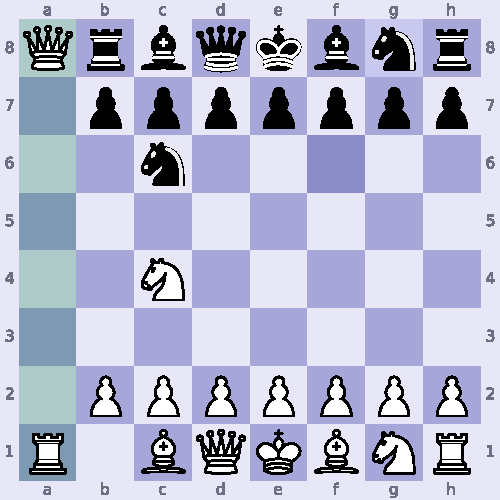
\includegraphics[width=\linewidth]{assets/board-cap10b}\\[2pt]
      \lccap{after a8=Q: six White}
    \end{column}
    \begin{column}{0.48\textwidth}
      \begin{lcstate}{Definition 3.2 · Lemma 3.3}{}
        {\small The two pawns starting on file $i$ are its \emph{origin
        pair}. If either ever makes a diagonal pawn move the file is
        \emph{resolved}, else \emph{unresolved}; write $f$ for the number of
        resolved files.\par\medskip
        \textbf{An unresolved pair makes at most $10$ pawn moves combined,
        and $10$ is attained.}}
      \end{lcstate}
      \begin{lcproof}
        {\small While both are on the board they stand on ranks $2+a$ and
        $7-b$ and cannot pass, so $2+a<7-b$, i.e.\ $a+b\le4$. Once one is
        captured (by some third piece) its contribution is frozen at
        $d\le4$ and the survivor has at most $6$ by Lemma 3.1:
        $d+6\le10$.\ \qed}
      \end{lcproof}
    \end{column}
  \end{columns}
  \par\vspace{0.1cm}
  {\small\color{lcaccent}\textbf{Remark 3.4.}
   ``Four combined'' holds only \emph{while both are on the board}.
   Used as a whole-game bound it excludes legal games.}
  \note{The two pawns that start facing each other on a file are that file's
  origin pair. If neither ever moves diagonally the file is unresolved, and
  $f$ counts the resolved files.

  While both are on the board they cannot pass. Capturing each other would
  need a diagonal move, excluded by assumption, and neither can overtake ---
  you cannot push onto an occupied square nor jump one with a double push.
  So four combined moves at most.

  But if one of them is captured by some \emph{other} piece, the survivor is
  free. On the left Black's a-pawn walks four squares and is taken by a
  knight; on the right White's a-pawn walks the whole file and promotes.
  Ten, not four.

  Remark 3.4 is in the paper for a reason: my own model got this wrong at
  one stage. Using four as a whole-game bound excludes legal games.}
\end{frame}

\begin{frame}{Proposition 3.6 --- $P - O \le 88$}
  \centering
  \vspace{0.15cm}
  \begin{columns}[c]
    \begin{column}{0.46\textwidth}\centering
      \figpminuso
    \end{column}
    \begin{column}{0.50\textwidth}
      \begin{lcstate}{Lemma 3.5}{overlap floor}
        {\small $O \ge f$. \ (For each resolved file pick one diagonal pawn
        move by a pawn of that origin file; distinct files have distinct
        movers, hence distinct overlaps.)}
      \end{lcstate}
      \begin{lcstate}{Proposition 3.6}{}
        {\small Since $P \le \min(96,\;80+2f)$,
        \[
          P - O \;\le\; \min(96,\,80+2f) - f \;\le\; \mathbf{88},
        \]
        with equality only at $f=8,\;P=96,\;O=8$.}
      \end{lcstate}
    \end{column}
  \end{columns}
  \par\vspace{0.25cm}
  {\small\color{lcaccent}
   Maximising over $f$ is what makes this a statement about \emph{every
   game} rather than about games that happen to have eight overlaps.}
  \note{Two ceilings.

  One: ten per unresolved file and twelve per resolved one, so $10(8-f) +
  12f = 80+2f$. The solid line.

  Two: six per pawn, 96 outright. The dashed line.

  But every resolved file contains at least one diagonal pawn move, which is
  a capture and hence an overlap, and different files contribute different
  moves. So $O \ge f$: resolving a file costs an overlap.

  Subtract and you get the thick line, peaking at 88 when $f$ is eight and
  strictly smaller everywhere else.

  Maximising over $f$ is the decisive step. Without it this would be a claim
  about one game rather than all of them.}
\end{frame}

\begin{frame}{Lemma 3.7 --- $C + T \le 30$}
  \centering
  \vspace{0.25cm}
  \begin{columns}[c]
    \begin{column}{0.28\textwidth}\centering
      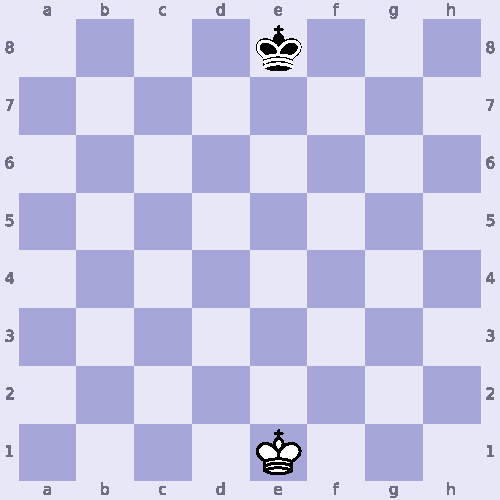
\includegraphics[width=0.88\linewidth]{assets/board-barekings}\\[3pt]
      \lccap{king against king: a dead position}
    \end{column}
    \begin{column}{0.66\textwidth}
      \begin{lcstate}{Lemma 3.7}{}
        {\small $C + T \le 30$.}
      \end{lcstate}
      \begin{lcproof}
        \begin{lcsteps}
          \item Only $30$ pieces are not kings, so $C \le 30$.
          \item If $C \le 29$ then $T \le 1$ gives $C+T \le 30$ at once.
          \item If $C = 30$, the thirtieth capture leaves the bare kings.
            King against king is a dead position, so the game ends on
            \emph{that} ply; no quiet ply follows and $T = 0$. \qedhere
        \end{lcsteps}
      \end{lcproof}
    \end{column}
  \end{columns}
  \par\vspace{0.3cm}
  {\small
   $\underbrace{96+30-8+0}_{\text{all 30 captured}} \;=\;
    \underbrace{96+29-8+1}_{\text{29, plus a closing segment}} \;=\; 118$
   \qquad neither route pays better.}
  \note{At most thirty captures, since kings are not capturable.

  But taking all thirty leaves the two kings alone, and king against king is
  a dead position --- no sequence of legal moves mates. So the game ends the
  instant it arises, nothing quiet can follow, and $T = 0$.

  Hence $C + T \le 30$. As the display shows, taking all thirty and losing
  the closing segment, or taking twenty-nine and gaining one, both give 118.

  Worth noting: this is the only place dead-position reasoning enters the
  bound at all, and king against king is the one case where deadness is
  beyond dispute.}
\end{frame}

\begin{frame}{Theorem 3.8 --- $K \le 118$}
  \centering
  \vspace{0.15cm}
  \begin{lcthm}{Theorem 3.8}{}
    \centering
    {\small Every game satisfies $K = (P-O)+(C+T) \le 88 + 30 =
    \mathbf{118}$. Moreover a game with $K = 118$ has
    $f = 8$, \ $P = 96$, \ $O = 8$, \ $C + T = 30$, so
    \emph{all sixteen pawns move six times and promote}, and $C \ge 29$.}
  \end{lcthm}
  \vspace{0.15cm}
  \begin{columns}[c]
    \begin{column}{0.30\textwidth}\centering
      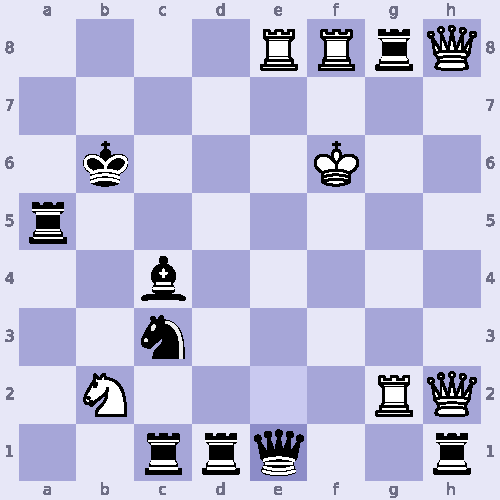
\includegraphics[width=0.86\linewidth]{assets/board-nopawns}\\[2pt]
      \lccap{the real game just after its last pawn move --- no pawns}
    \end{column}
    \begin{column}{0.64\textwidth}
      \begin{lcstate}{Remark 3.9}{Murphy's ceiling}
        {\small $K=118 \Rightarrow P=96 \Rightarrow$ both sides move pawns
        $\Rightarrow$ endpoints of both colours $\Rightarrow S \ge 1$, i.e.
        \[ L \;\le\; 150\cdot118 - 1 \;=\; 17{,}699. \]}
      \end{lcstate}
      {\small\color{lcaccent}The last two plies are the hard part, and
       Part III is nothing else.}
    \end{column}
  \end{columns}
  \note{Putting it together gives 118.

  The equality case is the useful part. To hit $88+30$ both halves must be
  tight, and Proposition 3.6's equality case pins $f$ at eight, $P$ at 96,
  $O$ at eight.

  As we saw, $P = 96$ means all sixteen pawns promoted. On the left is the
  real game just after its last pawn move: no pawns, and promoted rooks and
  queens everywhere. And $T \le 1$ gives $C \ge 29$.

  Remark 3.9 comes free. $P = 96$ means both sides move pawns, a pawn move is
  a critical move by its owner, so endpoints of both colours occur. The
  virtual endpoint is Black and some endpoint is White, so the colour
  changes at least once --- 17{,}699, Murphy's ceiling, now a theorem about
  all games.

  Remember two things: $P = 96$ and $C \ge 29$. Every argument in Part III
  runs on them.}
\end{frame}

% ====================================================== III. Switches
\lcpart{III}{Switches}{$K = 118$ forces $S \ge 3$}

\begin{frame}{Blocks and patterns}
  \centering
  \lcmap{3}
  \par\vspace{0.3cm}
  \begin{columns}[c]
    \begin{column}{0.53\textwidth}\centering
      \begin{tikzpicture}[x=1mm,y=1mm,font=\scriptsize]
        \foreach \c [count=\i from 0] in {B,B,B,W,W,B,B,W,W,W,W,B} {
          \path[seg\c] ({\i*6.2},0) rectangle ++(5.9,4.5);}
        \draw[lcarrow] (37,-3) -- (37,-9);
        \foreach \c/\s/\e in {B/0/2, W/3/4, B/5/6, W/7/10, B/11/11} {
          \path[seg\c,rounded corners=1pt]
            ({\s*6.2},-19) rectangle ({\e*6.2+5.9},-14);}
        \node[anchor=west,font=\tiny,text=lcgrey] at (78,2.2)
          {critical-move sequence};
        \node[anchor=west,font=\tiny,text=lcgrey] at (78,-16.5)
          {pattern $\B\W\B\W\B$};
      \end{tikzpicture}
    \end{column}
    \begin{column}{0.44\textwidth}
      \begin{lcstate}{Definition}{blocks · patterns}
        {\small Colour each critical move by whoever played it and group
        maximal single-colour runs into \emph{blocks}; the list of block
        colours is the \emph{pattern}. Doing the same to the endpoint
        sequence gives the \emph{endpoint pattern}.}
      \end{lcstate}
      \begin{lcstate}{Observation}{}
        {\small $n$ endpoint blocks $\Rightarrow$
        $S = n-1$ (opens Black) or $S = n$ (opens White).\par\medskip
        \textcolor{lcaccent}{So ruling out $S \le 2$ means killing every
        pattern of at most three blocks.}}
      \end{lcstate}
    \end{column}
  \end{columns}
  \note{One more piece of vocabulary.

  Colour each critical move by whoever played it --- a pawn move by the
  pawn's owner, a capture by the capturer.

  That gives a sequence of colours; group maximal runs of one colour into
  blocks and list the block colours, and you have the pattern. Top left is
  the sequence, below it the pattern.

  Do the same for endpoints and you get the endpoint pattern. With $n$
  blocks, $S$ is $n-1$ if it opens Black and $n$ if it opens White, because
  then it also disagrees with the virtual Black endpoint.

  So ruling out $S \le 2$ is exactly ruling out every pattern of at most
  three blocks.}
\end{frame}

\begin{frame}{There are exactly six patterns of at most three blocks}
  \centering
  \vspace{0.95cm}
  \figpatterns
  \par\vspace{1.05cm}
  {\small Kill all six and every pattern has at least four blocks,
   hence $S \ge 3$.}
  \note{A nonempty alternating pattern of at most three blocks is one of
  exactly six: B, W, BW, WB, BWB, WBW. That is the complete list.

  Show that none is possible at $K = 118$ and every pattern has at least
  four blocks, hence $S \ge 3$.

  The first four die by counting alone. The two three-block patterns are
  harder and need a lemma.

  To spoil the ending: the survivor is BWBW, and that is exactly the pattern
  of the real game.}
\end{frame}

\begin{frame}{Propositions 4.1 and 4.2 --- one and two blocks}
  \centering
  \vspace{0.1cm}
  \begin{columns}[t]
    \begin{column}{0.485\textwidth}
      \begin{lcstate}{Proposition 4.1}{one block}
        {\small $\B$ and $\W$ are impossible at $K=118$.\par\smallskip
        \emph{Proof.} If only one colour makes critical moves then only its
        eight pawns ever move, so $P \le 48 < 96$. \qed}
      \end{lcstate}
      \begin{lcstate}{Proposition 4.2}{two blocks}
        {\small $\B\W$ and $\W\B$ are impossible too.\par\smallskip
        \emph{Proof.} Write the pattern $(X,Y)$. Since $Y$ can capture only
        $X$'s $15$ capturable pieces, $C_Y \le 15$ and hence
        $C_X \ge 29-15 = 14$. Those $\ge14$ pieces are captured
        \emph{before} $Y$'s first critical move, so they never make a pawn
        move. At most $7$ of them did not begin as pawns, so $\ge7$ pawns
        lose all six of their moves. \qed}
      \end{lcstate}
    \end{column}
    \begin{column}{0.485\textwidth}\centering
      \vspace{0.2cm}
      \figtwoblocks
      \par\vspace{0.45cm}
      \scalebox{0.66}{\figpawngrid{6}{7}{54}}
    \end{column}
  \end{columns}
  \note{Proposition 4.1 is a single line. If only one colour ever makes a
  critical move then only its eight pawns ever move: $P \le 48$, and we need
  96.

  Proposition 4.2 is more interesting. Write the pattern $(X, Y)$: every
  critical move of $X$ precedes every critical move of $Y$.

  $Y$ can capture only $X$'s pieces, fifteen of them, so $C_Y \le 15$. Since
  $C \ge 29$, that leaves $C_X \ge 14$. The side moving first makes at least
  fourteen captures, all before $Y$ has made a single critical move.

  So those pieces were off the board before $Y$'s first critical move, which
  means they never made a pawn move at all. At most seven of them did not
  begin as pawns --- queen, two rooks, two bishops, two knights --- so at
  least seven pawns lose all six of their moves.

  That is the grid: forty-two cells gone, $P \le 54$, nowhere near 96.}
\end{frame}

\begin{frame}{Lemma 4.3 --- the home-rank lemma}
  \centering
  \vspace{0.15cm}
  \begin{columns}[c]
    \begin{column}{0.33\textwidth}\centering
      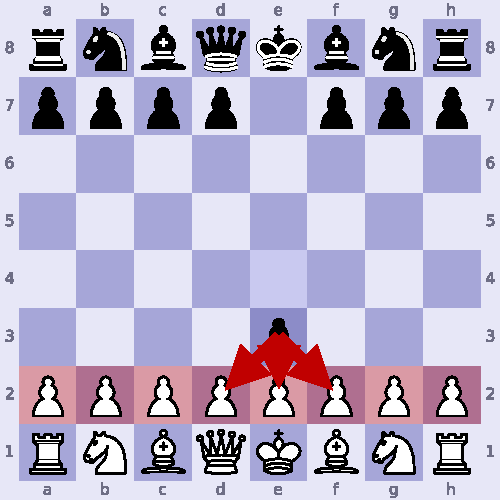
\includegraphics[width=0.92\linewidth]{assets/board-homerank}\\[2pt]
      \lccap{1.\,Nf3 e6\ 2.\,Ng1 e5\ 3.\,Nf3 e4\ 4.\,Ng1 e3}
    \end{column}
    \begin{column}{0.61\textwidth}
      \begin{lcstate}{Lemma 4.3}{home rank}
        {\small Fix an attacker $A$ and a defender $D$, and consider any
        position reachable from the initial one under
        \begin{itemize}\setlength{\itemsep}{1pt}
          \item[(R1)] every move by $D$ is quiet, and
          \item[(R2)] no move by $A$ captures a $D$ pawn.
        \end{itemize}
        Then $D$'s pawn home rank \emph{never changes}, no $A$ pawn ever
        stands on it, and \textcolor{lcaccent}{no $A$ pawn makes more than
        four pawn moves.}}
      \end{lcstate}
    \end{column}
  \end{columns}
  \par\vspace{0.25cm}
  {\small On the board Black's pawn stops on e3: only White may move the
   pawn on e2 (violating R1), and the only way through is capturing on d2 or
   f2 (violating R2).}
  \note{This is the heart of the paper.

  The setting: an attacker $A$ and a defender $D$, where $D$ plays only
  quiet moves and $A$ never captures a $D$ pawn.

  On the board, Black's pawn has walked four squares to e3 and stopped. It
  has nowhere to go.

  There is a White pawn on e2. Only White may move it, and moving a pawn is
  not a quiet move, so R1 forbids it. Black cannot push through because the
  square is occupied. Going round means capturing on d2 or f2, which is
  exactly what R2 forbids.

  So the home rank becomes a wall. Not one square of it ever changes.

  The rest of the proof, and why exactly four, is the next slide.}
\end{frame}

\begin{frame}{Proof of Lemma 4.3}
  \centering
  \vspace{0.15cm}
  \begin{columns}[c]
    \begin{column}{0.26\textwidth}\centering
      \fighomeranks
    \end{column}
    \begin{column}{0.68\textwidth}
      \begin{lcproof}
        \begin{lcsteps}
          \item \emph{$D$'s home rank never changes.} Induction over moves.
            No move can \emph{start} there --- the square holds a $D$ pawn
            and moving it violates (R1). None can \emph{end} there --- the
            square is occupied, so the move would be a capture, and $D$
            capturing violates (R1) while $A$ taking a $D$ pawn violates
            (R2). Castling touches only back ranks; en passant removes a
            pawn from rank $4$ or $5$.
          \item \emph{No $A$ pawn stands on $D$'s home rank.} A move ending
            there was ruled out in (1).
          \item \emph{Hence at most four moves.} The rank beyond is
            reachable only by a single step out of $D$'s home rank or a
            double push from a non-home rank, both impossible. The range is
            four ranks and each pawn move spends one. \qedhere
        \end{lcsteps}
      \end{lcproof}
    \end{column}
  \end{columns}
  \par\vspace{0.15cm}
  {\scriptsize\color{lcgrey}
   The induction uses only the elementary facts [H0]--[H6] about legal
   moves: what a move may change the occupancy of, and how a pawn advances.}
  \note{Once the wall is fixed, the rest is arithmetic.

  Step one is the wall. No move can start on those squares and none can end
  there. Castling and en passant are checked separately.

  Step two: an $A$ pawn cannot stand on $D$'s home rank, because a move
  ending there was just excluded.

  Step three: it cannot get past either. The rank beyond needs a single step
  out of $D$'s home rank --- which it can never occupy --- or a double push
  from somewhere that is not its own home rank, which the rules forbid.

  So the range is the four ranks between its home rank and $D$'s, and each
  pawn move spends at least one: four moves at most. And four is attained.}
\end{frame}

\begin{frame}{Proposition 4.4 --- three blocks $(X, Y, X)$}
  \centering
  \vspace{0.1cm}
  \begin{columns}[t]
    \begin{column}{0.50\textwidth}
      \begin{lcstate}{Proposition 4.4}{}
        {\small $\B\W\B$ and $\W\B\W$ are impossible at $K=118$.}
      \end{lcstate}
      \begin{lcproof}
        \begin{lcsteps}
          \item As before $C_Y \ge 14$, and all of these captures lie in
            the middle block. At least $7$ victims are $X$-pieces that
            began as pawns.
          \item All six pawn moves of such a piece $p$ fall \emph{before}
            $Y$'s first critical move $\tau$: any $X$-critical move after
            $\tau$ belongs to the final block, which is after $p$ was
            captured.
          \item The first phase is exactly Lemma 4.3's setting --- (R1) by
            the definition of $\tau$, (R2) from $P=96$. So each $X$ pawn
            gets at most \emph{four} moves there. \qedhere
        \end{lcsteps}
      \end{lcproof}
    \end{column}
    \begin{column}{0.47\textwidth}\centering
      \vspace{0.15cm}
      \figthreeblocks
      \par\vspace{0.2cm}
      \scalebox{0.58}{\figpawngrid{2}{7}{82}}
    \end{column}
  \end{columns}
  \note{Now the three-block case.

  Step one is as before: $C_Y \ge 14$, and all of $Y$'s critical moves lie
  in the middle block, so all of those captures do too. At least seven
  victims are $X$ pieces that began as pawns.

  Step two: take one of them, $p$. It must make six pawn moves, all before
  it is captured. But any critical move by $X$ after $Y$'s first one --- ply
  $\tau$ --- belongs to the final $X$ block, which comes after $p$ was
  taken. A piece off the board cannot move. So all six fall in the first
  phase.

  Step three: the first phase is exactly the lemma's setting. R1 is
  immediate from the definition of $\tau$; R2 comes from $P = 96$, because a
  captured $Y$ pawn would make no pawn move at all.

  So each $X$ pawn gets at most four moves where six are needed. Seven pawns
  short by two gives $P \le 82$.}
\end{frame}

\begin{frame}{Theorem 4.5 --- $S \ge 3$}
  \centering
  \vspace{0.45cm}
  \begin{lcthm}{Theorem 4.5}{four blocks}
    \centering
    {\small Every game with $K = 118$ has a critical-move pattern of at
    least four blocks. The endpoint sequence is that sequence with at most
    one element appended, which cannot lower the block count, so the
    endpoint pattern has at least four blocks too and $\;S \ge 3$.}
  \end{lcthm}
  \vspace{0.5cm}
  \begin{tikzpicture}[x=1mm,y=1mm,font=\scriptsize]
    \node[lcbox] (a) at (0,0) {$\B$, $\W$\\ Prop.~4.1};
    \node[lcbox] (b) at (32,0) {$\B\W$, $\W\B$\\ Prop.~4.2};
    \node[lcboxa] (c) at (66,0) {$\B\W\B$, $\W\B\W$\\ Prop.~4.4};
    \node[lcboxk] (d) at (104,0) {$\ge4$ blocks\\ $S \ge 3$};
    \draw[lcarrow] (a) -- (d); \draw[lcarrow] (b) -- (d);
    \draw[lcarrow] (c) -- (d);
  \end{tikzpicture}
  \par\vspace{0.5cm}
  {\small\color{lcgrey}
   \textbf{Remark 4.6.} $S \ge 3$ holds \emph{only} under $K = 118$.
   Repeating 1.\,Nf3 Nf6 2.\,Ng1 Ng8 four times gives a 16-ply game with
   $K = 1$ and $S = 0$.}
  \note{All six are dead, so the pattern has at least four blocks.

  The endpoint sequence is the critical-move sequence with at most one
  element appended, and appending cannot reduce the block count. So the
  endpoint pattern also has at least four blocks, and $S \ge 3$.

  Remark 4.6 deserves emphasis. $S \ge 3$ is conditional on $K = 118$ and
  nothing else. In general it is plainly false: repeat Nf3 Nf6 Ng1 Ng8 four
  times and the game ends after sixteen plies by fivefold repetition of the
  initial position, with no pawn move and no capture, so $K = 1$ and
  $S = 0$.

  That costs nothing, because a game with $K \le 117$ has already forfeited
  a whole segment and no switch count makes that back.}
\end{frame}

\begin{frame}{Theorem 5.1 --- the upper bound}
  \centering
  \vspace{0.4cm}
  \begin{lcthm}{Theorem 5.1}{upper bound}
    \centering No legal chess game lasts more than $17{,}697$ plies.
  \end{lcthm}
  \vspace{0.3cm}
  \begin{lcproof}
    {\small
    \begin{tabular}{@{}ll@{}}
      $K \le 117$ & Lemma 2.4 with $S \ge 0$: \
                    $L \;\le\; 150 \cdot 117 \;=\; 17{,}550 \;<\; 17{,}697$ \\[5pt]
      $K = 118$   & the largest Theorem 3.8 permits; Theorem 4.5 gives
                    $S \ge 3$, so \
                    $L \;\le\; 150 \cdot 118 - 3 \;=\; \mathbf{17{,}697}$ \\
    \end{tabular}\par\medskip
    \hfill\qed}
  \end{lcproof}
  \vspace{0.3cm}
  \begin{lcthm}{Corollary 5.3}{exact maximum}
    \centering
    {\small The bound is attained (Labelle's generated game, Murphy's
    hand-built one). \textbf{The maximum length of a chess game is exactly
    $17{,}697$ plies --- $8{,}848$ moves and one final White ply.}}
  \end{lcthm}
  \note{The proof is two lines.

  If $K \le 117$ a whole segment is missing, so $L \le 150 \times 117 =
  17{,}550$, less than 17{,}697.

  If $K = 118$, the theorem we just proved gives $S \ge 3$, so $L \le 150
  \times 118 - 3 = 17{,}697$.

  Keeping the cases separate is the point: $S \ge 3$ is not available below
  118 and is not needed there either --- one segment outweighs any switch
  count.

  And the lower bound already exists: two published games are exactly this
  long. So the maximum is exactly 17{,}697 --- an equality, not an
  inequality.}
\end{frame}

\begin{frame}{Corollary 5.2 --- the structure of a maximum-length game}
  \centering
  \vspace{0.5cm}
  \begin{lcthm}{Corollary 5.2}{}
    \centering
    {\small Every game of length $17{,}697$ satisfies
    $K = 118$, \ $S = 3$, \ every $\delta_i = 0$, \
    $f = 8$, \ $P = 96$, \ $O = 8$, \ $C + T = 30$, and both its
    critical-move and endpoint patterns are $\B\W\B\W$.}
  \end{lcthm}
  \vspace{0.5cm}
  {\small
  all sixteen pawns move six times, one rank each, and promote
  \quad$\cdot$\quad every segment is full ($150$, or $149$ across a
  change)}
  \par\vspace{0.55cm}
  {\large \lcstrip{B,W,B,W}\ \ $\B\W\B\W$ \quad
   \textcolor{lcaccent}{Black makes the first critical move, and the final
   endpoint is White's.}}
  \note{The equality analysis costs nothing extra.

  If the length is 17{,}697 then every inequality above was an equality. So
  $K = 118$, $S$ is exactly three, and every $\delta$ is zero --- not one
  segment wasted.

  All the equality conditions follow: sixteen pawns promoted, exactly eight
  overlaps.

  The pattern is pinned too. There are exactly four blocks, and it cannot
  open with White --- that would disagree with the virtual Black endpoint as
  well and force $S \ge 4$. So it is BWBW.

  Which means we know what a maximum-length game looks like. Black makes the
  first critical move; White plays the last. There is no choice about it.}
\end{frame}

% ======================================================== IV. Search
\lcpart{IV}{Search}{what came before the theorem}

\begin{frame}{Search 1 --- brute variety}
  \centering
  \lcmap{4}
  \par\vspace{0.35cm}
  \figattackone
  \par\vspace{0.45cm}
  {\small Same $118$ critical moves, freshly generated quiet filler, many
   distinct $17{,}697$-ply games $\rightarrow$ test every one for a single
   additional legal ply}
  \note{Chronologically this came first. I was trying to break 17{,}697.

  The first attempt was the blunt one: start from the known game, keep its
  118 critical moves, regenerate all the quiet filler between them, and
  mass-produce distinct 17{,}697-ply games. One of them differs from the
  original in 17{,}032 of its plies.

  Then ask every one of them the same question: can you add one more legal
  ply?

  Never. Every game hit exactly the same wall.

  That is not a proof, but it was the signal that the wall was not an
  accident.}
\end{frame}

\begin{frame}{Search 2 --- targeted search}
  \centering
  \vspace{0.55cm}
  \figattacktwo
  \par\vspace{1.05cm}
  {\small Hypothesis: \emph{a legal skeleton keeps $118$ segments while
   switching the acting colour at most twice}}
  \par\vspace{0.45cm}
  {\color{lcaccent}\small An abstract CP-SAT model over pawn-move and
   capture budgets, plus a planner to realise candidates as real moves ---
   every instance infeasible}
  \note{The second attempt had a target: there is a legal skeleton with 118
  segments that switches the acting colour at most twice.

  I built an abstract CP-SAT model over the pawn-move and capture budgets,
  and a concrete planner to turn any candidate into an actual sequence of
  moves.

  Every instance came back infeasible. The planner never had anything to do.

  That is where I turned around. Failing to find something repeatedly can
  mean it is not there. I stopped treating 17{,}697 as a target to beat and
  started treating it as a theorem to prove.}
\end{frame}

\begin{frame}{The structure of the proof}
  \centering
  \vspace{0.9cm}
  \figdag
  \par\vspace{1.1cm}
  {\small Not one line of this needs a computer.}
  \note{And this is the shape the proof took. On the left the elementary
  lemmas about pawns and captures, in the middle $K \le 118$, on the right
  the pattern argument and $S \ge 3$.

  The box underneath is the $K \le 117$ case, which simply runs out of
  segments at 17{,}550.

  The point: none of this needs a computer. All of it is checkable by hand.
  The computer appears in the next part, and what it does there is
  cross-check, not replace.}
\end{frame}

% ====================================================== V. Checking
\lcpart{V}{Checking}{computation does not replace the proof}

\begin{frame}{What the computation does}
  \centering
  \lcmap{5}
  \par\vspace{0.75cm}
  \figpipeline
  \par\vspace{0.95cm}
  {\small Above: judge the game \quad$\cdot$\quad
   Below: cross-check the hand argument by two independent methods
   (sound direction only --- only infeasibility is used)}
  \note{The computer does two things.

  Above the line: an independent verifier replays Murphy's game from the
  initial position, ply by ply. Legality, whether anything terminates early,
  a classification of the position after every ply --- and it passes a
  sequence only if the game ends exactly on its last move. That verifier
  imports nothing else from the repository, so the judge shares no code with
  any producer of games.

  Below the line: every finite case analysis is exhausted mechanically, and
  the pattern question --- does any endpoint pattern of at most three blocks
  admit $K = 118$? --- is decided twice more, by a CP-SAT model and by a
  solver-free arithmetic checker that declares its own constants.

  Both are used in the sound direction only. Infeasible means no such game
  exists; feasible does not mean one does. No claim in the paper rests on a
  feasibility verdict.}
\end{frame}

\begin{frame}{Two rules the verifier implements}
  \centering
  \vspace{0.6cm}
  \begin{columns}[t]
    \begin{column}{0.47\textwidth}
      \begin{lcstate}{Mate outranks the clock}{}
        {\small The final ply is the $150$th quiet ply of its segment
        \emph{and} a checkmate (the precedence clause of
        Art.~9.6.2).\par\medskip
        A verifier that consults the clock first accepts the same
        $17{,}697$ plies but \alert{scores the game a draw.}}
      \end{lcstate}
    \end{column}
    \begin{column}{0.47\textwidth}
      \begin{lcstate}{Never compare whole FENs}{}
        {\small For repetition the clock and move number play no part in
        identity, and en passant counts only when \emph{legal}
        (Art.~9.2).\par\medskip
        \alert{Naive keys fail both ways} --- a FEN over-distinguishes;
        placement plus side to move ignores castling rights and
        over-merges.}
      \end{lcstate}
    \end{column}
  \end{columns}
  \par\vspace{0.7cm}
  {\small Under that identity no position of this game occurs even
   \emph{three} times --- fivefold repetition is never approached.}
  \note{These are rules of chess, not engineering choices, and the reference
  game exercises both.

  First, the order of the termination tests. The final ply is simultaneously
  the 150th quiet ply of its segment and a checkmate; the precedence clause
  keeps the mate. A verifier that looks at the clock first accepts the same
  17{,}697 plies but records a draw --- right length, wrong result.

  Second, position identity for repetition. Do not compare whole FEN
  strings: the halfmove clock and move number play no part in identity, and
  the en passant target is written after every double push whether or not a
  capture is legal, so fivefold would never fire. Comparing only placement
  and side to move goes wrong the other way, ignoring retained castling
  rights.

  As an aside, Tom 7's reference implementation still has MOVE\_RULE set to
  50 directly beneath a comment saying 75 is correct. A reference
  implementation is not an oracle --- which is why ours is independent.}
\end{frame}

\begin{frame}{Verdict and reproduction}
  \centering
  \vspace{0.65cm}
  {\small
  \begin{tabular}{@{}ll@{}}
    \toprule
    the game & legal, $17{,}697$ plies, ends in checkmate \\
    early termination & none --- no position occurs even three times, no
                        stalemate \\
    profile & $K = 118$, $P = 96$, $C = 29$, $O = 8$, $T = 1$, $S = 3$
              --- exactly Corollary 5.2 \\
    decomposition & $115 \times 150 \;+\; 3 \times 149 \;=\; 17{,}697$,
                    \ $\sum_i \delta_i = 0$ \\
    pattern & endpoint pattern $\B\W\B\W$ \\
    cross-check & all six patterns of $\le3$ blocks infeasible, both
                  methods agree \\
    \bottomrule
  \end{tabular}}
  \par\vspace{0.85cm}
  {\small A second game is verified the same way --- same $118$ critical
   moves, fresh filler, $17{,}032$ plies differ.}
  \par\vspace{0.3cm}
  {\scriptsize\color{lcgrey}
   Everything re-runs from a byte-for-byte reproducible certificate:
   \texttt{make verify-full}}
  \note{The verification in one table.

  The game is legal, 17{,}697 plies, ends in checkmate. Nothing terminates
  early --- the clock stays under 150 after every ply but the last, and no
  position ever occurs even three times.

  And the profile is exactly what Corollary 5.2 forces. The decomposition
  closes exactly: 115 segments of 150, three of 149, nothing wasted.

  Here is the thing worth saying out loud: improving on such a game is not
  hard, it is impossible. Every segment is full, and the three plies it
  loses are exactly the three the theorem proves unavoidable.

  So that the result does not rest on a single artefact, a different game of
  the same length was rebuilt and verified the same way.}
\end{frame}

% ====================================================== VI. Meaning
\lcpart{VI}{Meaning}{one game, and a sequence that stops}

\begin{frame}{The reference game's segment structure}
  \centering
  \lcmap{6}
  \par\vspace{0.75cm}
  \figsegments
  \par\vspace{0.55cm}
  \figsegmentskey
  \par\vspace{0.5cm}
  {\small one bar per segment \quad$\cdot$\quad
   colour is the endpoint's colour \quad$\cdot$\quad
   \textcolor{lcaccent}{the three $149$s sit exactly on the block
   boundaries}}
  \note{This is the game. One bar per segment, all 118, taken from the
  actual PGN rather than drawn as a schematic.

  A bar's colour is the colour of that segment's endpoint, so the four
  visible runs are the BWBW pattern: ten Black, forty-nine White, fifty
  Black, nine White.

  The strip along the bottom says what ended each segment --- a pawn move, a
  capture, or both. Ninety-six pawn moves, twenty-nine captures, eight
  overlaps, one closing segment. The whole count, visible.

  And the three marked in red are the 149s. Look at where they are: exactly
  on the block boundaries. Segments eleven, sixty and a hundred and ten. One
  ply lost wherever the colour changes.

  What we proved today is that those three cannot be two.}
\end{frame}

\begin{frame}{Corollary --- A048987 has finite support}
  \centering
  \vspace{0.4cm}
  \figoeis
  \par\vspace{0.7cm}
  \begin{lcstate}{}{OEIS A048987}
    \centering
    {\small The sequence counting chess games that end at ply $n$ has
    \textbf{finite support}, with last nonzero term $a(17697)$.}
  \end{lcstate}
  \par\vspace{0.3cm}
  {\scriptsize\color{lcgrey}The curve is schematic --- the true $a(n)$ runs
   to $10^{29241}$ and beyond (Labelle).}
  \note{Another way to state the result.

  OEIS A048987 counts chess games that end at ply $n$. What we proved is
  that this sequence has finite support, and that its last nonzero term is
  exactly $a(17697)$.

  Read the curve for shape only. The real values are enormous --- Labelle's
  Monte Carlo estimate puts the total above $10^{29241}$. Treat the vertical
  axis as ``nonzero''.

  That chess is finite has been known since 2014. What today adds is where
  it stops.}
\end{frame}

\begin{frame}{Open directions}
  \centering
  \vspace{0.55cm}
  \begin{columns}[t]
    \begin{column}{0.31\textwidth}
      \begin{lcstate}{Parameter}{}
        {\small The maximum as a function of the ``$n$-move rule''. The
        ``three'' in this argument uses the fact that $75$ is odd.}
      \end{lcstate}
    \end{column}
    \begin{column}{0.31\textwidth}
      \begin{lcstate}{Abstraction}{}
        {\small Games with a bounded stock of counter-resetting events ---
        does the same accounting hold away from chess?}
      \end{lcstate}
    \end{column}
    \begin{column}{0.31\textwidth}
      \begin{lcstate}{Formalisation}{}
        {\small The counting proof in a proof assistant, and
        re-verification under an independently implemented move generator.}
      \end{lcstate}
    \end{column}
  \end{columns}
  \par\vspace{1.05cm}
  \lcquote{The upper bound is a hand-checkable combinatorial theorem. The
    lower bound is a previously known explicit construction.\\[2pt]
    \emph{Computation verifies the construction and cross-checks the proof;
    it does not replace it.}}{}
  \note{Three directions and then I will stop.

  One. Replace 75 by $n$ and ask for the answer as a function of $n$. The
  ``three'' here uses that 75 is odd; the even case is separate.

  Two. Abstraction: games with a finite stock of counter-resetting events
  --- does the same accounting go through away from chess?

  Three. Formalisation. This is a counting proof, a good shape for a proof
  assistant. And we currently trust python-chess's move generation;
  re-verifying under an independent implementation would shrink that trust.

  One last sentence. The upper bound is a hand-checkable theorem, the lower
  bound is a construction that already existed, and computation verifies the
  construction and cross-checks the proof without replacing it. Thank you.}
\end{frame}

\begin{frame}{References}
  \centering
  \vspace{-0.15cm}
  \begin{columns}[t]
    \begin{column}{0.58\textwidth}
      {\scriptsize
      F.~Labelle, \emph{The longest possible chess game, and bounds on the
        number of possible chess games}, 2015.
        \texttt{wismuth.com/chess/longest-game.html}\\[3pt]
      T.~Murphy~VII, \emph{Is this the longest Chess game?}, SIGBOVIK 2020,
        pp.~20--31.\\[3pt]
      O.~Heimo, \emph{Pisin shakkipeli}, Suomen Tehtäväniekat 58(4--5),
        2004.\\[3pt]
      E.~Bonsdorff, K.~Fabel, O.~Riihimaa, \emph{Schach und Zahl},
        Walter Rau, 1971.\\[3pt]
      M.~Euwe, \emph{Mengentheoretische Betrachtungen über das Schachspiel},
        KNAW 32, 1929.\\[3pt]
      FIDE, \emph{Laws of Chess}, Handbook E/01, in force 2023.\\[3pt]
      Ing Chess (developer of Augment Chess), \emph{The theoretically
        longest chess game}. YouTube channel --- see QR
        \,$\cdot$\, \texttt{augmentchess.org}\\[3pt]
      J.~Yim, companion repository (v1.0.0, Zenodo DOI).
        \texttt{github.com/junyeobe0315/long\_chess}}
      \par\vspace{0.4cm}
      {\scriptsize\textbf{Thanks.} Tom Murphy VII and François Labelle,
      with the forum contributors Deedlit, Tatzelwurm and Falkenbach, for
      the construction and the question; Alexis Langlois-Rémillard for
      comments on the draft; and Ing Chess, whose video started all of
      this.}
    \end{column}
    \begin{column}{0.38\textwidth}\centering
      \begin{tabular}{@{}c@{\quad}c@{\quad}c@{}}
        \qrcode[height=1.8cm]{https://github.com/junyeobe0315/long_chess} &
        \qrcode[height=1.8cm]{https://wismuth.com/chess/longest-game.html} &
        \qrcode[height=1.8cm]{https://www.youtube.com/@\%EC\%9E\%89\%EC\%B2\%B4\%EC\%8A\%A4} \\[3pt]
        {\tiny repository} & {\tiny Labelle} & {\tiny Ing Chess} \\
      \end{tabular}
      \par\vspace{0.4cm}
      \lcshot{2.4cm}{assets/shot-sigbovik.png}{[SIGBOVIK 2020]}\\[2pt]
      {\tiny\color{lcgrey}Murphy VII, SIGBOVIK 2020}
    \end{column}
  \end{columns}
  \note{References and thanks.

  This work exists because Tom Murphy VII built the game and asked the
  question. The numbers behind the answer --- the 118 and the three-switch
  structure --- were found years earlier by François Labelle and the forum
  contributors his page credits. What I added is the proof that it is
  optimal.

  The three codes are the repository, Labelle's page, and the Ing Chess
  channel where this problem started. The repository has the paper, the
  verifier and a reproducible certificate; one make verify-full re-runs all
  of it in about twenty seconds.

  Questions.}
\end{frame}

\end{document}
